\chapter{Competitive Programming Problems}
\section{Common function functions }
This section describes the utility functions that are used to write solution for the followings problems.

\begin{lstlisting}[language=c++, caption="For each functions"]

template <typename Iterator, typename Lambda>
void for_each(Iterator s, Iterator e, Lambda l) {
  while (s != e) {
    l(*s);
    s++;
  }
}

//Lambda has type (T& -> int -> void)
template <typename Container, typename Lambda>
void for_each_i(Container& v, const int s, const int e, Lambda l) {
    int i=s;
    while (i < e){
        l(v[i],i);
        i++;
    }
}
	\end{lstlisting}
	
	
	
\begin{lstlisting}[language=c++, caption="Store credit c++ solution"]

template <typename T, typename Iterator>
bool contains(const Iterator s, const Iterator e, const T& value) {
  auto predicate_equal = [&](T curr) { return value == curr; };
  bool ret = e == find_if(s, e, predicate_equal);
  return !ret;
}

// Return value
// Iterator to the first element satisfying the condition or last if no such
// element is found.
template <typename Iterator, typename Lambda>
Iterator find_if(Iterator s, Iterator e, Lambda predicate) {
  while (s != e) {
    if (predicate(*s))
      return s;

    s++;
  }
  return e;
}

// Return value
// Iterator to the first element satisfying the condition or last if no such
// element is found.
template <typename Iterator, typename Lambda>
inline Iterator find_if_not(Iterator s, Iterator e, Lambda predicate) {
  auto not_predicate = [&](auto v) { return !predicate(v); };
  return find_if(s, e, not_predicate);
}

	\end{lstlisting}



\begin{lstlisting}[language=c++, caption="Store credit c++ solution"]
template <typename Iterator, typename Lambda>
bool all_of(Iterator s, Iterator e, Lambda predicate) {
  while (s != e) {
    if (!predicate(*s))
      return false;
    s++;
  }
  return true;
}

template <typename Iterator, typename Lambda>
bool any_of(Iterator s, Iterator e, Lambda predicate) {
  while (s != e) {
    if (predicate(*s))
      return true;
    s++;
  }

  return false;
}
\end{lstlisting}





\begin{lstlisting}[language=c++, caption="Store credit c++ solution"]
// Lambda has type: D -> T -> D
template <typename D, typename Iterator, typename Lambda>
D fold(Iterator s, Iterator e, const D& a, Lambda l) {
  D acc = a;
  while (s != e) {
    acc = l(acc, *s);
    s++;
  }
  return acc;
}

\end{lstlisting}


\begin{lstlisting}[language=c++, caption="Read input functions"]
template <typename T>
void readVector(std::vector<T>& v, const int size, std::istream& is=std::cin) {
  LOOPUP(i, size) {
    T a;
    is >> a;
    v.push_back(a);
  }
}

template <typename T, unsigned int D>
void readArray(std::array<T, D>& v, std::istream& is=std::cin) {
  LOOPUP(i, D) {
    T a;
    is>> a;
    v[i] = a;
  }
}


void read(auto& v, const unsigned int size, std::istream& is=std::cin) {
    using T=typename std::remove_reference<decltype(v[0])>::type;
  LOOPUP(i, size) {
    T a;
    is>> a;
    v[i] = a;
  }
}
\end{lstlisting}


\begin{lstlisting}[language=c++, caption="Store credit c++ solution"]
template<typename T>
inline T safe_midpoint(const T lo, const T hi){
    return lo+(hi-lo)/2;
}


template<typename T>
inline T unsafe_midpoint(const T lo, const T hi){
    return (hi+lo)/2;
}


template<typename T>
inline bool lt(const T& v1,const T& v2){
    return v1 < v2;
}

template<typename T>
inline bool eq(const T& v1,const T& v2){
    return v1 == v2;
}

template<typename T>
inline bool gt(const T& v1,const T& v2){
    return v1 > v2;
}

template<typename T>
inline bool gte(const T& v1,const T& v2){
    return gt(v1,v2) || eq (v1,v2);
}
template<typename T>
inline bool lte(const T& v1,const T& v2){
    return lt<T>(v1,v2) || eq<T>(v1,v2);
}

\end{lstlisting}




\begin{problem}{\textit{Store Credit} - \textbf{Google Jam Qualification Round Africa 2010}}
You receive a credit C at a local store and would like to buy two items. You first walk through the store and create a list L of all available items. From this list you would like to buy two items that add up to the entire value of the credit. The solution you provide will consist of the two integers indicating the positions of the items in your list (smaller number first).

\textbf{Input}

The first line of input gives the number of cases, N. N test cases follow. For each test case there will be:
One line containing the value C, the amount of credit you have at the store.
One line containing the value I, the number of items in the store.
One line containing a space separated list of I integers. Each integer P indicates the price of an item in the store. Each test case will have exactly one solution.

\textbf{Output}

For each test case, output one line containing "Case \#x: " followed by the indices of the two items whose price adds up to the store credit. The lower index should be output first.
\begin{framed}
	\begin{verbatim}
Input 
3
100
3
5 75 25
200
7
150 24 79 50 88 345 3
8
8
2 1 9 4 4 56 90 3

Output 
Case #1: 2 3
Case #2: 1 4
Case #3: 4 5
	\end{verbatim}
\end{framed}

\end{problem}

\begin{solution}
	
	\begin{lstlisting}[language=c++, caption="Store credit c++ solution"]

#include<common.h>
using namespace std;

int main(){
    using P=pair<int,int>;
    int N; cin>>N;

    LOOPUP(i,N){
        int C; cin>>C;
        int I; cin>>I;
        vector<int> items(I);
        vector<P> ip(I);
        DS::read(items,I);
        DS::for_each_i(ip,0,I,
            [&](auto& el, const int idx){el.first=items[idx]; el.second=idx;}
        );

        DS::quicksort(ip,0,I,DS::lt<P>);
        auto eq_fn = [](const P& p, const int v){ return p.first==v; };
        auto cmp_fn = [](const P& p, const int v){ return p.first<v; };
        LOOPUP(j,ip.size()){
            int val = (C-items[j]);
            int idx = DS::binary_search_idx(ip,0,ip.size(), val ,eq_fn,cmp_fn);
            //found. pickup the one with lowest INDEX
            if(idx!= -1){
                int retidx =idx;
                bool good=false;//check we do not pickup the same element twice
                while(eq_fn(ip[retidx],val) && j!= ip[retidx].second ){
                    retidx--;
                    good=true;
                }
                if(good){
                    int l = j+ 1;
                    int h = ip[retidx+1].second+1;
                    cout<<"Case #"<<i+1<<": "<<min(l,h)<<" "<<max(l,h)<<endl;
                    int sum = items[j] + items[ip[retidx+1].second];
                    assert(sum==C);
                    break;
                }
            }
        }
    }//foreach testcase
    return 0;
}

	\end{lstlisting}
\end{solution}





\begin{problem}{\textit{Rope Intranet} - \textbf{Google Jam Round 1C 2010}}

A company is located in two very tall buildings. The company intranet connecting the buildings consists of many wires, each connecting a window on the first building to a window on the second building.

You are looking at those buildings from the side, so that one of the buildings is to the left and one is to the right. The windows on the left building are seen as points on its right wall, and the windows on the right building are seen as points on its left wall. Wires are straight segments connecting a window on the left building to a window on the right building.

You've noticed that no two wires share an endpoint (in other words, there's at most one wire going out of each window). However, from your viewpoint, some of the wires intersect midway. You've also noticed that exactly two wires meet at each intersection point.

On the above picture, the intersection points are the black circles, while the windows are the white circles.

How many intersection points do you see?

\begin{figure}
\centering
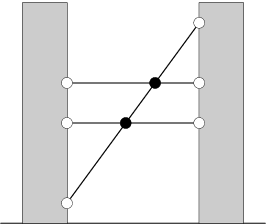
\includegraphics[scale=1]{ropeinternet}
\caption{}
\label{fig:ropeinternet}
\end{figure}

You've noticed that no two wires share an endpoint (in other words, there's at most one wire going out of each window). However, from your viewpoint, some of the wires intersect midway. You've also noticed that exactly two wires meet at each intersection point.

On figure \ref{fig:ropeinternet}, the intersection points are the black circles, while the windows are the white circles.

How many intersection points do you see?



\textbf{Input}
The first line of the input gives the number of test cases, T. T test cases follow. Each case begins with a line containing an integer N, denoting the number of wires you see.

The next N lines each describe one wire with two integers Ai and Bi. These describe the windows that this wire connects: Ai is the height of the window on the left building, and Bi is the height of the window on the right building.


\textbf{Output}
For each test case, output one line containing "Case \#x: y", where x is the case number (starting from 1) and y is the number of intersection points you see.

\begin{framed}
	\begin{verbatim}
Input 
2
3
1 10
5 5
7 7
2
1 1
2 2

Output 
Case #1: 2
Case #2: 0
	\end{verbatim}
\end{framed}

\end{problem}

\begin{solution}
	
	\begin{lstlisting}[language=c++, caption="Store credit c++ solution"]


	\end{lstlisting}
\end{solution}




\begin{problem}{\textit{Rope Intranet} - \textbf{Google Jam Round 1C 2010}}




\textbf{Input}


\textbf{Output}


\begin{framed}
	\begin{verbatim}
Input 


Output 

	\end{verbatim}
\end{framed}

\end{problem}

\begin{solution}
	
	\begin{lstlisting}[language=c++, caption="Store credit c++ solution"]


	\end{lstlisting}
\end{solution}




\begin{problem}{\textit{Rope Intranet} - \textbf{Google Jam Round 1C 2010}}




\textbf{Input}


\textbf{Output}


\begin{framed}
	\begin{verbatim}
Input 


Output 

	\end{verbatim}
\end{framed}

\end{problem}

\begin{solution}
	
	\begin{lstlisting}[language=c++, caption="Store credit c++ solution"]


	\end{lstlisting}
\end{solution}



\begin{problem}{\textit{Rope Intranet} - \textbf{Google Jam Round 1C 2010}}




\textbf{Input}


\textbf{Output}


\begin{framed}
	\begin{verbatim}
Input 


Output 

	\end{verbatim}
\end{framed}

\end{problem}

\begin{solution}
	
	\begin{lstlisting}[language=c++, caption="Store credit c++ solution"]


	\end{lstlisting}
\end{solution}



\begin{problem}{\textit{Rope Intranet} - \textbf{Google Jam Round 1C 2010}}




\textbf{Input}


\textbf{Output}


\begin{framed}
	\begin{verbatim}
Input 


Output 

	\end{verbatim}
\end{framed}

\end{problem}

\begin{solution}
	
	\begin{lstlisting}[language=c++, caption="Store credit c++ solution"]


	\end{lstlisting}
\end{solution}



\begin{problem}{\textit{Rope Intranet} - \textbf{Google Jam Round 1C 2010}}




\textbf{Input}


\textbf{Output}


\begin{framed}
	\begin{verbatim}
Input 


Output 

	\end{verbatim}
\end{framed}

\end{problem}

\begin{solution}
	
	\begin{lstlisting}[language=c++, caption="Store credit c++ solution"]


	\end{lstlisting}
\end{solution}



\begin{problem}{\textit{Rope Intranet} - \textbf{Google Jam Round 1C 2010}}




\textbf{Input}


\textbf{Output}


\begin{framed}
	\begin{verbatim}
Input 


Output 

	\end{verbatim}
\end{framed}

\end{problem}

\begin{solution}
	
	\begin{lstlisting}[language=c++, caption="Store credit c++ solution"]


	\end{lstlisting}
\end{solution}